

Having derived the theoretical predictions given by our model, we can take a final step forward by comparing these results with the observational data we presented in chapter \ref{chap:halos}. In particular, we choose to focus on the ALMA ALPINE sample described in section \ref{sec:alpine} (for the original paper, see F20 \citep{Fujimoto:2020qzo}). We select this sample because it is the only study of \CII spatial emission in individual high-z galaxies. \CII emission profiles from individual galaxies are very useful because they allow a comparison between the parameters in our model and the properties of the galaxies considered in the sample. 

The F20 study identifies -- from the original ALPINE sample of 23 galaxies whose \CII emission is located above the $5\sigma$ level -- seven different systems that fall into their "\CII halo" category. By considering this subset of profiles, we run our model with different parameters in order to compare it with the data.
%
Our aim is twofold: on the one hand, we want to use this comparison to determine whether there is good accordance between our theoretical framework and observations. If that were the case, we would have a quantitative argument in favor of the outflows hypothesis as the best candidate to explain the origin of \CII halos.
%
On the other hand, it is interesting to use the data to gauge the values of the parameters in our model. Assuming that outflows are indeed the main source for these high-z halos, in fact, we can draw some interesting conclusions on the physical conditions of high-z galaxies by inferring the best-fit values of the parameters of our model. 

In this chapter, we focus on these different tasks. We start by studying whether our model is able to account for the \CII emission measured by observations (section \ref{sec:single_profiles_comp}). Then, we set up a Markov Chain Monte Carlo (MCMC) simulation in order to infer the posterior probability distribution for the parameters in our model (section \ref{sec:mcmc}). Finally, in section \ref{sec:results}, we discuss our results, also in light of previous theoretical and observational work. 


\section{Comparison with individual profiles} \label{sec:single_profiles_comp}

\subsection{Description of the sample} \label{sec:sample_description}

The sample of "CII Halo" systems identified by F20 consists of seven different galaxies with the following property: considering the emission coming only from a peripheral region (i.e., masking the central galaxy's contribution), the statistical significance of the \CII line must be above the $4\sigma$ level, and, at the same time, (rest-frame) UV and FIR continuum must be below $3\sigma$. To this sample, we add the system DC$494057$, which does not belong to the "\CII Halo" category in F20 as it does not respect the bounds on the FIR/UV continuum luminosities. However, this system has been studied by HC21 \citep{herrera2021kiloparsec} in a follow-up work (sec. \ref{sec:alpine}), showing clear evidence for the presence of a \CII halo and an outflow. 

By combining ALMA observations with ancillary data coming from HST, VLT, and Spitzer, it is possible to measure the different properties of these systems. In particular, the \CII line can give an estimate of the redshift, $z = z_\mathrm{CII}$, and the combined measurements of rest-frame UV and FIR continuum allow a Spectral Energy Distribution (SED) fitting that gives an estimate both of the star formation rate (SFR) and of the stellar mass ($M_\mathrm{star}$). As described in the last chapter, $z$ and $\mathrm{SFR}$ are important parameters in our model. Therefore, these ancillary data can be used to constraint the parameter space we have described in section \ref{sec:outflow_profiles}. 

Another very important quantity that determines the evolution of the wind in our model is the halo virial mass $M_\mathrm{vir}$ (or, equivalently, the global circular velocity $v_c$; see sec. \ref{sec:cooling_gravity}). The halo mass can be linked to the stellar mass via a redshift-dependent function, known as the Stellar Mass-Halo Mass relation (SMHM).
%
As described in section \ref{sec:feedback}, this relation depends on a number of physical processes that are quite difficult to model. However, it is possible to gauge this relation by combining semi-analytical prescriptions for the halos and galaxies growth with observables such as the galaxy luminosity function, the star formation rate history, etc.
%
A great deal of theoretical work has focused on this task, obtaining a satisfactory description of how the SMHM relation evolves with redshift. Here, we use the modeling by \citet{behroozi2013average} to link the stellar mass to the virial mass and to the global circular velocity.

In table \ref{tab:alpine_sample}, we show the properties of the eight systems considered. Overall, these systems are normal, $z \approx 4.5-5.5$, star-forming galaxies, with star formation rates between $10$ and $100\,\msun\,\mathrm{yr}^{-1}$, stellar masses in the range $0.5-1.5 \,\times10^{10}\,\msun$, and, consequently, global circular velocities around $200-250\,\kms$.

\begin{table}
\centering
%
\begin{tabular}{ c c c c c c }
\hline
Name   & $z$    & $\mathrm{SFR}$ [$\msun\,\mathrm{yr}^{-1}$]   & $M_\mathrm{star}$ [$10^{9}\,\msun$]    & $M_{vir}$ [$10^{11}\,\msun$]     & $v_c$ [$\mathrm{km}\,\mathrm{s}^{-1}$] \\ 
\hline
\hline
DC$396844$    &    $4.54$    &    $55^{+40}_{-25}$    &   $7.3^{+2.6}_{-2.6}$   &   $4.1^{+2.8}_{-1.8}$    &   $206^{+90}_{-66}$ \\
DC$494057$   & $5.54$   &    $42^{+35}_{-15}$    &   $14.2^{+4.9}_{-4.2}$   &   $6.7^{+5.2}_{-3.5}$    &   $263^{+133}_{-97}$\\
DC$630594$    &    $4.44$    &    $31^{+24}_{-15}$    &   $5.9^{+2.3}_{-1.7}$   &   $3.6^{+2.6}_{-1.5}$    &   $196^{+85}_{-59}$ \\
DC$683613$    &    $5.54$    &    $58^{+44}_{-26}$    &   $14.7^{+5.7}_{-4.4}$   &   $7.0^{+5.9}_{-3.7}$    &   $267^{+145}_{-102}$ \\
DC$880016$    &    $4.54$    &    $32^{+25}_{-15}$    &   $5.6^{+2.3}_{-1.6}$  &   $3.5^{+2.6}_{-1.4}$    &   $196^{+85}_{-58}$ \\
DC$881725$    &    $4.58$    &    $88^{+61}_{-43}$    &   $9.1^{+4.0}_{-2.1}$   &   $4.8^{+3.5}_{-2.1}$    &   $217^{+98}_{-68}$  \\
VC$5100537582$    &    $4.55$    &   $15^{+14}_{-6}$    &   $5.7^{+2.0}_{-1.6}$  &   $ 3.6^{+2.5}_{-1.5}$    &   $197^{+83}_{-58}$ \\
VC$5110377875$    &    $4.55$    &    $99^{+79}_{-41}$    &   $14.7^{+4.7}_{-5.6}$   &   $7.0^{+5.1}_{-3.9}$    &   $246^{+125}_{-97}$ \\
 \hline
\end{tabular}
%
\caption{Properties of the "CII Halo" sample taken from the F20 study \citep{Fujimoto:2020qzo}. From left to right: name of the ALPINE source ("DC" stands for "DEIMOS COSMOS", while "VC" stands for "VUDS COSMOS"), redshift ($z$), Star Formation Rate ($\mathrm{SFR}$), stellar mass ($M_\mathrm{star}$), halo mass ($M_{vir}$), and global circular velocity ($v_c$). Uncertainties on the redshift measurements are very small and not shown here. 
\label{tab:alpine_sample}
}
\end{table}

\subsection{$\chi^2$ test} \label{sec:chi2}

\begin{figure*}[t]
    \centering
    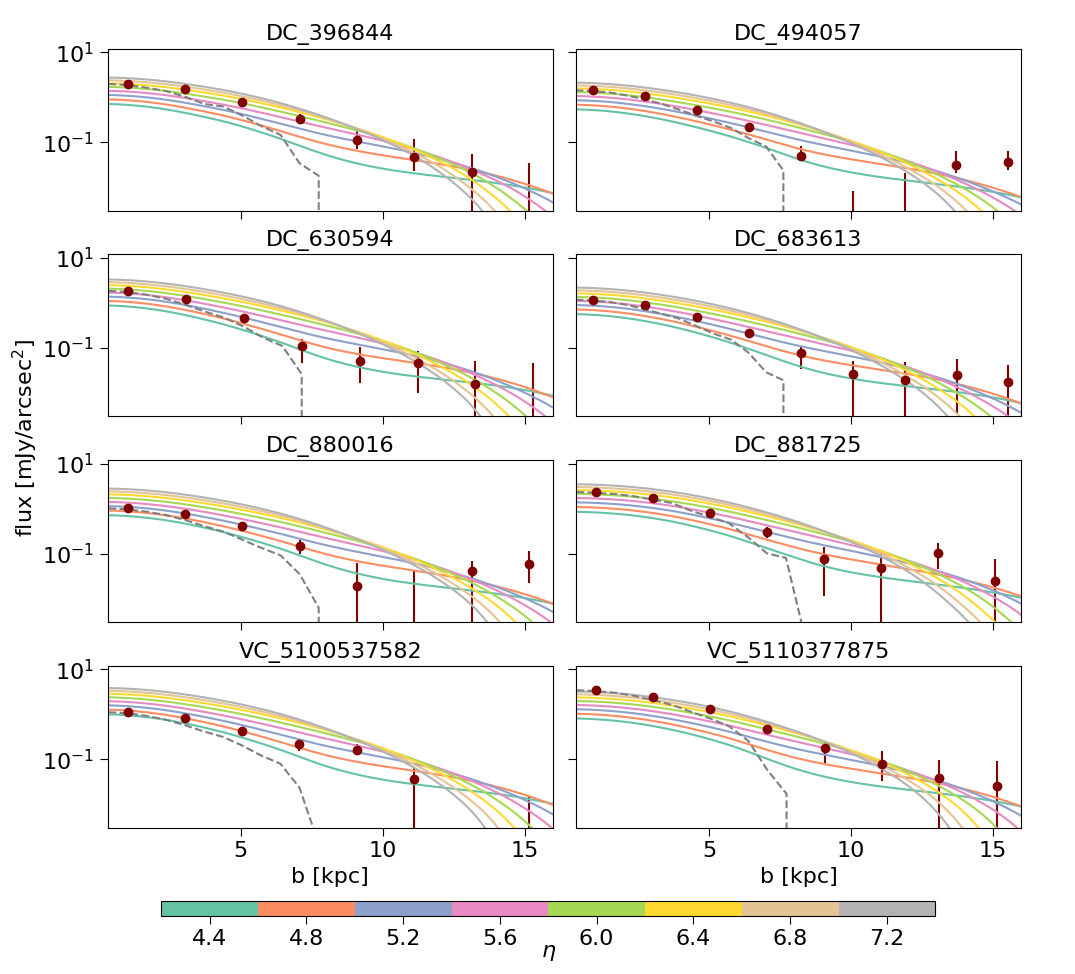
\includegraphics[width=1.0\textwidth]{plots/single_profile_emission.png}
    \caption{Comparison of the \CII profiles obtained by using the model presented in chapter $\ref{chap:model}$ (colored lines) with data from the F20 "\CII Halo" sample (red dots). All parameters are fixed according to observations (table \ref{tab:alpine_sample}), except for the mass loading factor $\eta$ which is varied in the plots. The profiles are convolved with the same beams as in the observations (shown with dashed grey lines in the plots).
    \label{fig:single_profiles}
    }
\end{figure*}


\begin{table}
\centering
%
\begin{tabular}{ c c c }
\hline
Name      & $\chi^2_\mathrm{min}(d|\eta)$  & $\eta_\mathrm{min}$  \\ 
\hline
\hline
DC$396844$      &    $12.6$  &    $5.5$ \\
DC$494057$      &    $8.6$  &    $8.4$ \\
DC$630594$      &    $20.9$ &    $6.4$  \\
DC$683613$      &    $3.6$ &    $5.3$   \\
DC$880016$     &    $10.0$  &    $5.9$  \\
DC$881725$    &    $17.5$  &    $4.0$    \\
VC$5100537582$   &   $16.9$   &    $8.2$   \\
VC$5110377875$    &    $45.6$  &    $4.3$   \\
 \hline
\end{tabular}
\caption{Results for the $\chi^2$ test for the F20 \citep{Fujimoto:2020qzo} (sub-)sample here considered. ALPINE source names are listed in the first column (see also table \ref{tab:alpine_sample}); the second column refers to the minimum value of $\chi^2(d|\eta)$ with respect to the mass loading factor, whose minimizing value $\eta_\mathrm{min}$ is shown in the third column. Details of the model-data comparison can be found in the text and in figure \ref{fig:single_profiles}. 
\label{tab:alpine_chi2}
}
\end{table}

For each system, we can take as fiducial value the one obtained by table \ref{tab:alpine_sample}. As a result, if we also assume (as argued in section \ref{sec:outflow_profiles}) $Z= 1\,Z_\odot$ and $\fesc=0$, the only residual parameter in our model is the mass loading factor $\eta$. For this reason, as a first investigation, we study how the model compares with the data for different values of the $\eta$ parameter. Figure \ref{fig:single_profiles} shows how our model compares with the F20 sample: observational data are plotted, together with the emission profiles resulting from our outflow model, for different values of $\eta$. These profiles are created by using the observational estimates for redshift, SFR, circular velocity, and FWHM of the \CII line, and they are also convolved with the same beam as observations. 

Almost all the plots in figure \ref{fig:single_profiles} indicate a good level of accordance between the data and our model. To base our comparison on quantitative arguments, we introduce a $\chi^2$ statistics as a measure of the "\textit{goodness of fit}" for our theoretical model. The $\chi^2$ for a set of $n$ data $d=\{y_i(x_i)\pm\sigma_i\}_{i=1}^n$ and a model $m$ (depending on a parameter $\eta$), is defined as:
\begin{align}
    \chi^2(d | \eta ) = \sum_{i=1}^n \frac{(y_i - m(x_i;\eta))^2}{\sigma_i^2}
\end{align}
If we assume that: (a) different measurements are independent; (b) the errors $\sigma_i$ have Gaussian distributions; and (c) the errors on the quantities $x_i$ are negligible; then, we expect the random variable $\chi^2(d | \theta )$ to be distributed just as a $\chi^2$ with $n-1$ degrees of freedom (i.e., as a squared sum of $n-1$ normal Gaussian variables). A $\chi^2$ with $n-1$ degrees of freedom has an expectation value $E(\chi^2) = n-1$, and a variance $\sigma^2({\chi^2})=2(n-1)$.

For the F20 sample, the hypotheses on which the $\chi^2$ test is founded are valid. Therefore, running the test on the sample, we should recover in principle extractions from a $\chi^2$ distribution with a number of data per set of $n=9$. However, we caution the reader that this discussion has some limitations. In fact, we do not expect the results of a $\chi^2$ test to be fully accurate in the case here considered, for a variety of reasons. Most importantly, our model has several limitations: many assumptions we have made (e.g., spherical symmetry, time stationarity, very crude treatment of the central galaxy) are expected to cause important variations on the data profiles and/or fluctuations. %Therefore, we need to be aware of the limitations of our model when interpreting how it compares with data.

For instance, the fact that the central emission is not well modeled in our framework has important consequences in the computation of the $\chi^2$, as the errors of the central data points are the smallest ones (because of their higher S/N). Thus, even profiles that, overall, are in good agreement with the data can have a relatively high $\chi^2$. Further discussion on limitations and possible improvements is left for the final chapter (chap. \ref{chap:conclusion}). Nonetheless, the values of the $\chi^2$ can be considered as a first, approximated way to determine whether there are values of $\eta$ for which the accordance of the model with the F20 profiles reach a satisfactory level. With this respect, we display in table \ref{tab:alpine_chi2} the minimum value of $\chi^2(d|\eta)$ for each of the F20 profiles considered, and the corresponding value of the $\eta$ parameter which corresponds to  $\chi^2_\mathrm{min}(d|\eta)$.

For most of the systems, good accordance is found between the model and the data profile for values of $\eta$ ranging from $\eta\approx 4$ o $\eta \approx 8$.
%
The only notable exception is VC$5110377875$: in this case, the flux in the central region is particularly intense, and the only values of $\eta$ that are compatible with similar values of the emission in the central regions are $\eta \approx 7-8$; these same values, however, are not compatible with the extension of the halo in the external regions of the CGM, as they are slowed down by gravity and their emission drops at distances that are too small compared with the data. In the same way, lower values of $\eta$ are too faint for the central emission but are faithfully representing the outer regions of the halo. With this respect, we note that a missing contribution from the central ISM (discussed at the end of section \ref{sec:CII_emission}) could alleviate the conflict between model and data. 

\subsection{$\mathrm{SFR}$ and $v_c$ dependences}

\begin{figure*}
    \centering
    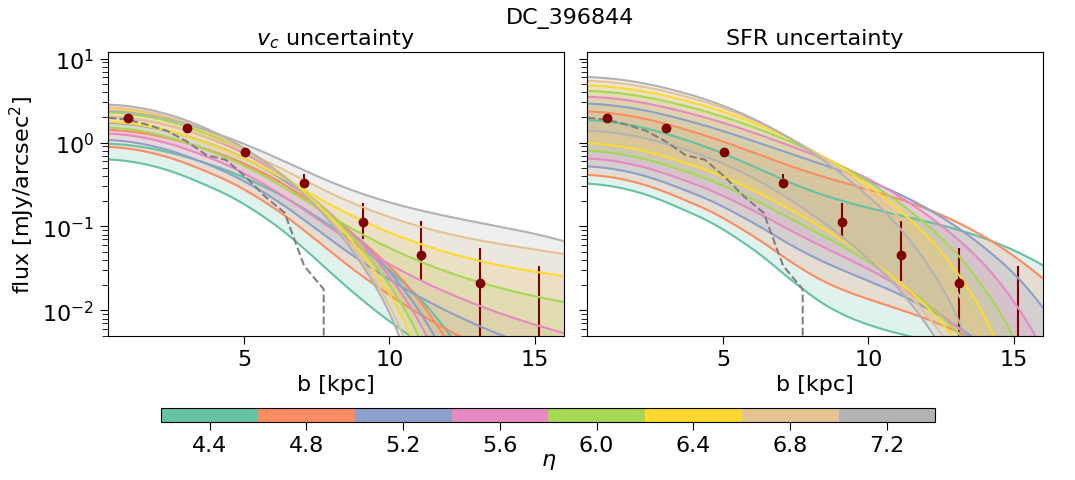
\includegraphics[width=1.0\textwidth]{plots/vc_sfr_emission.png}
    \caption{Same comparison between theoretical profiles and observational data, as in figure \ref{fig:single_profiles}. The DC$396844$ system is considered for illustrative purposes. \textit{Left}: the lower and higher limits for the global circular velocity $v_c$ -- as inferred from observations -- are considered. All the other parameters are fixed to their observational best estimate (table \ref{tab:alpine_sample}), while the mass loading factor $\eta$ is varied in the plot. For every value of $\eta$, the profiles corresponding to $v_{c,\mathrm{min}}$ and $v_{c,\mathrm{max}}$ are plotted, and the region between them is shaded accordingly. \textit{Right}: same as the left panel, but the star formation rate is considered. Profiles are created by setting the SFR equals to $\mathrm{SFR}_\mathrm{max}$ and $\mathrm{SFR}_\mathrm{min}$, as inferred by observations (table \ref{tab:alpine_sample}). 
    \label{fig:sfr_vc_unc}
    }
\end{figure*}

The $\chi^2$ analysis has shown that a good fraction of the systems considered is well-fitted by our single-parameter models. We could go further in our analysis by studying, e.g., the error associated with the best-fit values of $\eta$. However, we choose to follow another approach, as we realize that a single-parameter model has some intrinsic limitations that can bias our final results.
%
The reason for that can be appreciated by looking at table \ref{tab:alpine_sample} (see also figure \ref{fig:alpine_trends}): the relative errors on the values of the circular velocity and the star formation rate, as derived from observations, are as high as $50 \%$ both for $v_c$ and SFR -- redshift measurements, instead, are very precise.
%
Such uncertainties can have significant implications for our choice of parameters. We can appreciate this by studying the dependence of the final emission profiles on $v_c$ and on $\mathrm{SFR}$. 

Changing the value of $v_c$ is equivalent to modifying the gravitational pull acting on the outflowing gas. This alters the evolution of the wind quite considerably: increasing $v_c$, the gas velocity $v$ decreases (in particular in the outer regions), and, consequently, its density $n$ tends to increase. Ultimately, these changes result in a smaller stalling radius $r_\mathrm{stop}$, and hence in a different extension of the gaseous halo formed by the wind.
%
The effects of these changes on the final, convolved, \CII emission profiles are quite difficult to quantify, as opposite trends are at play: higher densities imply a higher \CII emission, but at the same time, smaller stalling radii results in an emission that drops earlier and thus it is not as strong in the outer regions of the CGM.

In order to see whether these expected trends have a measurable impact on our final results, we study how $v_c$ affects the final \CII emission profiles in figure \ref{fig:sfr_vc_unc} (left panel). In particular, we consider the same \CII emission profiles that we have shown in figure \ref{fig:single_profiles}, i.e., focusing on the system DC$396844$.
%
In this case, however, we consider different values for the circular velocity $v_c$: we plot the lower and the upper fiducial bounds that can be inferred from observations (table \ref{tab:alpine_sample}). We highlight the differences between these two choices by filling in the region between the two profiles. As in figure \ref{fig:single_profiles}, we repeat this procedure for different choices of the mass loading factor $\eta$, color-coding the results accordingly. The resulting plot implies that, indeed, our model is quite sensitive to the value of the global circular velocity selected, and observations alone cannot provide us with the best choice for $v_c$ because of the relatively large uncertainties of the measurements. 

These conclusions are even more dramatic if we consider the dependence of the \CII profiles on the star formation rate. For $\fesc = 0$, the set of equations governing the wind evolution (eqs.\ref{eq:cooling_model_equations}) does not depend on the SFR. Even so, the SFR affects the outflow profiles because it determines the boundary conditions for the wind (eqs. \ref{eq:boundary}).
%
In particular, it holds: $n(R) \propto \mathrm{SFR}\,\eta^{3/2}$. As the density is the most important quantity determining the final \CII emission, changing the SFR is expected to have similar effects as changing the mass loading factor $\eta$. The right panel of figure \ref{fig:sfr_vc_unc} validates these expectations: as done for $v_c$, we plot the \CII emission profiles for the system DC$396844$ setting $\mathrm{SFR}_\mathrm{min}$ and $\mathrm{SFR}_\mathrm{max}$ as inferred by observations (table \ref{tab:alpine_sample}). Given the large relative uncertainties on SFR measurements, the data fall mostly inside the shaded regions for all the $\eta$ values considered. 

The analysis here presented suggests that it is necessary to expand the parameter space considered in the comparison with data, in particular including the star formation rate and the global circular velocity as parameters; this is the goal of the next section, where we still use observations to guide our exploration of the parameter space, but we do not restrict ourselves to fixed values of $\mathrm{SFR}$ and $v_c$.

\section{MCMC analysis} \label{sec:mcmc}

\begin{figure*}
    \centering
    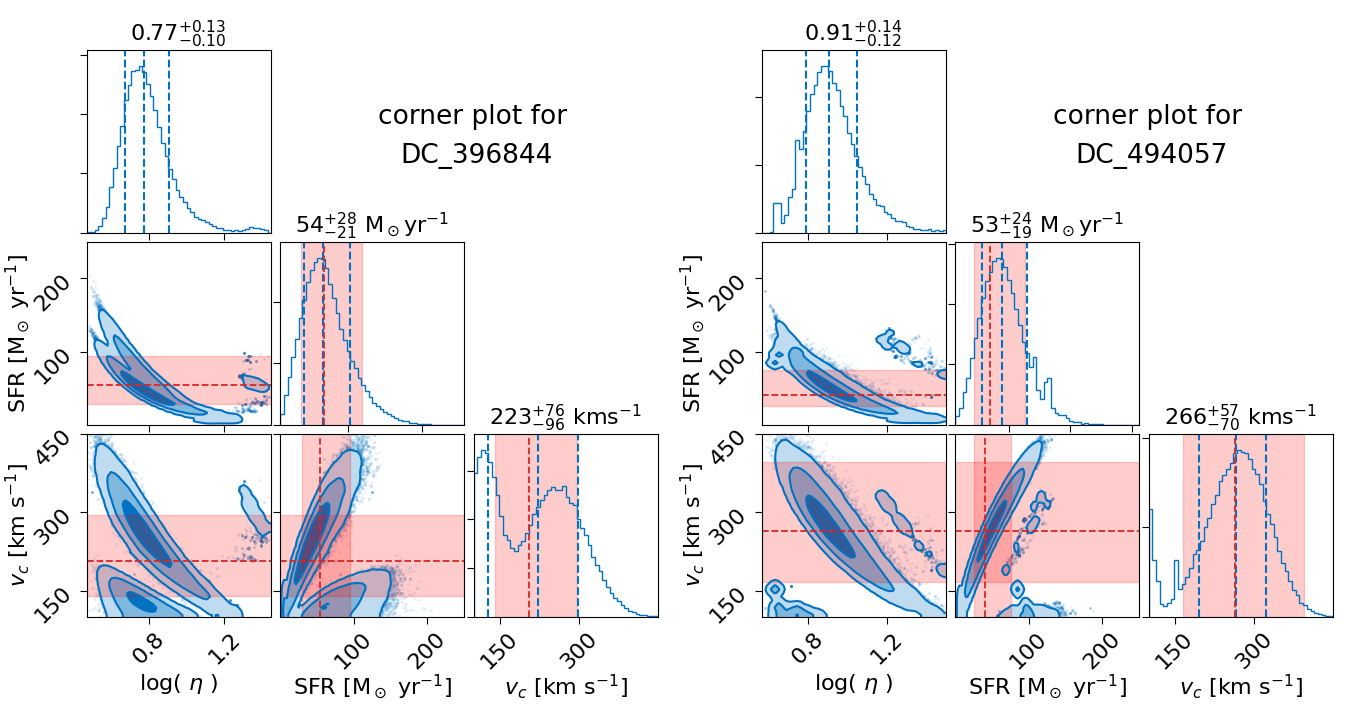
\includegraphics[width=1.0\textwidth]{plots/corner_final_1.png}
    \caption{Corner plots (i.e., 1-d and 2-d marginalizations) of the 3-d posterior distribution $P(\Theta|d,m)$, with $\Theta = \{\log\eta, \mathrm{SFR}, v_c\}$. The posterior distribution was sampled using an MCMC algorithm, set up with the Python package \code{emcee} (details in the text). Two out of the eight F20 "\CII Halo" systems are shown here (the other ones are shown in figure \ref{fig:corner_2}). The values of the parameters $\mathrm{SFR}$ and $v_c$, as inferred from observations (table \ref{tab:alpine_sample}), are shown with red dashed lines, together with their uncertainties (red shaded regions). The blue dashed vertical lines represent the median and $1\sigma$ errors on the parameters: these same quantities are also shown at the top of each 1-d histogram. 
    \label{fig:corner_1}
    }
\end{figure*}

From the discussion in the last section, it follows that the parameter space needs to be extended by including $\mathrm{SFR}$ and $v_c$. In principle, we could minimize the new, multi-dimensional $\chi^2$ distribution $\chi^2(d|\eta, \mathrm{SFR}, v_c)$ to find the best-fitting parameters, just as we did in section \ref{sec:single_profiles_comp}.
%
However, it is convenient at this point to introduce a more general framework for two main reasons: (a) we still want to exploit in our analysis the values of the star formation rates and of the global circular velocity inferred from observations; (b) we want to associate an uncertainty to the best-fitting values of the parameters.

\subsection{The Bayesian framework} \label{sec:bayes}

The setting of the Bayesian framework is the same we have already considered in section \ref{sec:single_profiles_comp}: a theoretical model $m(\Theta)$ (depending on a set of parameters $\Theta$) is to be compared with some data $d=\{y_i(x_i)\pm \sigma_i\}$.
%
In the Bayesian approach, however, the question one seeks to answer is different: which is the probability distribution associated with the set of parameters $\Theta$ that can be inferred from the comparison with data?
%
Bayes theorem allows to write this distribution (known as "posterior"), $P(\Theta|d,m)$, in terms of two other quantities: a "prior" distribution $\pi(\Theta|m)$, expressing the a-priori (i.e., not coming from the data) information on the parameters, and a "likelihood" $\mathcal{L}(d|\Theta,m)$, describing the probability of obtaining the set of data $d$ assuming a fixed set of parameters $\Theta$. The Bayes theorem reads:
\begin{equation}
    P(\Theta\,|d,m) = \frac{\pi(\Theta|m)\,\mathcal{L}(d\,|\Theta, m)}{\mathcal{Z}(d|m)},
\end{equation}
where $\mathcal{Z}(d|m)= \int \d \Theta\,\pi(\Theta)\,\mathcal{L}(d\,|\Theta, m) $ (dubbed as "evidence") can be considered a normalization constant.

Under the same hypotheses as section \ref{sec:chi2} (i.e., independence between different measurements, Gaussianity of statistical errors), it can be proven \citep[e.g.,][]{jaynes_2003} that the likelihood is a function of $\chi^2$:
\begin{equation}
    \mathcal{L}(d\,|\Theta, m) = e^{-\chi^2(d|\Theta)} = \exp\left(-\sum_{i=1}^n \frac{(y_i - m(x_i;\eta))^2}{\sigma_i^2}\right)
\end{equation}
Therefore, maximizing the likelihood is the same as minimizing the $\chi^2$: in this sense, the Bayesian approach and the $\chi^2$ formalism are equivalent. An important difference, however, is played by the prior term $\pi(\Theta|m)$. In fact, this quantity can alter the final shape of the posterior distribution in a way that the $\chi^2$ approach is not able to capture. 

In this analysis, we have chosen to focus on three parameters: the mass loading factor $\eta$, the star formation rate (SFR), and the global circular velocity $v_c$. Therefore, we need to specify the priors for these quantities.
%
The a-priori knowledge we have on these parameters varies. The mass loading factor is largely unconstrained both theoretically and observationally: even its order of magnitude is quite unclear, ranging from $\eta \lesssim 0.1$ to $\eta \gtrsim 10$ \citep[e.g.,][]{muratov2015}. For this reason, the most suitable prior for $\eta$ is a logarithmic prior (i.e., a uniform prior for $\log \eta$). Therefore, from now on we work with the parameter $\log \eta$, assigning to it a uniform prior in the range $-1 < \log\eta < 1.5$. On the other hand, both $\mathrm{SFR}$ and $v_c$ are constrained by our general knowledge of high-z galaxies; moreover, the ancillary data in table \ref{tab:alpine_sample} give even more accurate estimates for their values. For this reason, we choose to set Gaussian priors for these two quantities, centered in their fiducial values inferred from observations, and with a standard deviation equal to half of the total (upper+lower) error of these measured values.

Overall, the prior distribution we consider is null outside the region $-1 < \log\eta < 1.5$, while inside this region it equals to ($\Delta(\log\eta) = 2.5$):
\begin{equation}
    \pi(\Theta|m) =  \frac{1}{\Delta(\log\eta)}\frac{1}{2\pi\sigma_{\mathrm{SFR},i}\sigma_{v_c,i}}\exp\left(-\frac{\left(\mathrm{SFR}-\mathrm{SFR}_i\right)^2}{2\sigma_{\mathrm{SFR},i}^2}-\frac{\left(v_c-v_{c,i}\right)^2}{2\sigma_{v_c,i}^2}\right),
\end{equation}
where $\mathrm{SFR}_i \pm \sigma_{\mathrm{SFR},i}$ and $v_{c,i} \pm \sigma_{v_c,i}$ refers to the values displayed in table \ref{tab:alpine_sample}.

\subsection{Setting up MCMC runs}

\begin{figure*}[t]
    \centering
    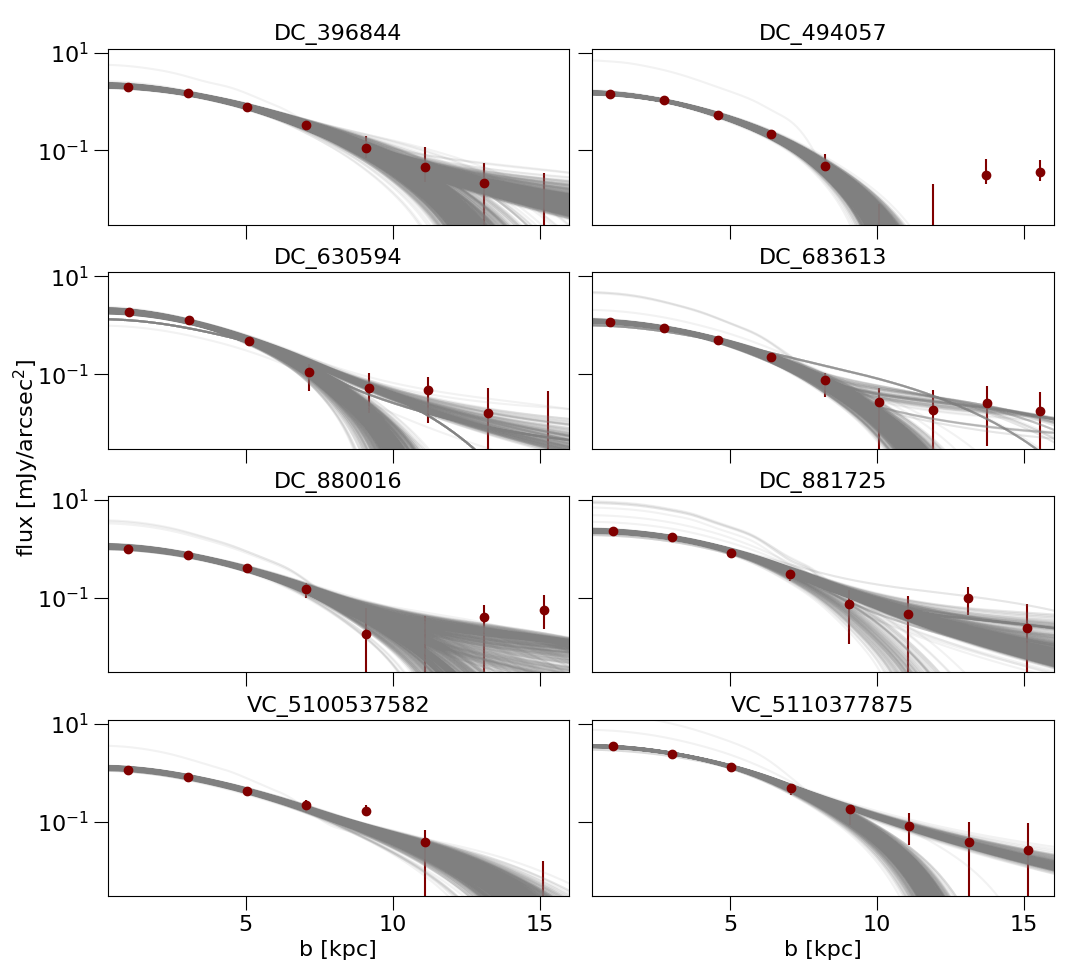
\includegraphics[width=1.0\textwidth]{plots/mcmc_emission.png}
    \caption{Comparison of the \CII profiles obtained by using the model presented in chapter $\ref{chap:model}$ (light gray lines) with data from the F20 "\CII Halo" sample (red dots). The profiles are created by choosing $10^3$ different values of the parameters, extracting them randomly from the MCMC chains ($\{\Theta_i\}_{i=1}^N$) obtained in section \ref{sec:mcmc}. The profiles are convolved with the same beams as in the observations (shown in figure \ref{fig:single_profiles}).
    \label{fig:mcmc_emission}
    }
\end{figure*}

Once the priors are set, the posterior distribution is well-defined, and it can be computed at any point of the parameter space. The most naive approach that can be followed to describe the global behavior of the posterior is to build a grid in the parameter space and to compute the posterior for every point in the grid. However, this approach gets more and more problematic as the dimensions of the parameter space increase. Already in 3-D, techniques based on stochastic samplers become competitive. The idea behind this alternative approach is to generate a list of $N$ posterior samples $\{\Theta_i\}_{i=1}^N$ drawn from the parameter space, such that the number of samples on the region $\Theta + \Delta \Theta$ ($\Delta \Theta \ll \Theta$) is proportional to $P(\Theta|d,m)$. 

The most popular class of samplers is represented by the Markov Chain Monte Carlo (MCMC) algorithms \citep{metropolis, hastings}. In MCMC methods, a set of $m$ particles (dubbed as "walkers") move randomly in the parameter space. At each step, the probability for a particle to move to any given point is determined by a Markov chain, that is created following several possible prescriptions; these prescriptions aim to generate new samples according to the posterior distribution.
%
By recording the positions of the walkers at each iteration, "chains" of elements $\{\Theta_i\}_{i=1}^N$ are created. These chains can be thought of as draws from the posterior probability distribution; therefore, a simple histogram of the elements in the chains reveals the shape of the posterior. Of course, the first elements of every chain need to be discarded because they depend on the chain's initial conditions (this is the so-called "burn-in" phase). Additionally, there are inevitable correlations between the position of a walker at a given step in the chain and its positions at the following/preceding steps. These correlations can be averaged to give the "autocorrelation time" $\tau$. It is important to check that this autocorrelation time does not exceed a small fraction of the full length of the chain; if it does, its effects need to be accounted for, as the width of the distribution gets underestimated because of correlations.

%It is also beneficial to run many different walkers starting from different regions of the parameter space, as a single walker can fail to find multiple modes of a posterior distribution if there are regions of low posterior probability between the modes. 

Here, we do not describe the details of different algorithmic prescriptions, nor do we analyze the many other subtleties that must be considered when dealing with MCMC samplers \citep[for a review on this, see e.g.,][]{sharma2017markov}. Instead, we limit ourselves to describe the general setup that we choose for our analysis: we use the well-known code \code{emcee} \citep{foreman2013emcee} to run an MCMC using the affine-invariant ensemble prescription to generate new samples \citep{goodman_prescription}. For each system considered (table \ref{tab:alpine_sample}), we run the MCMC algorithm by placing $m=96$ walkers distributed randomly in the parameter space and evolving them for $N=10^5$ steps. We discard the first $10^3$ elements to account for the burn-in phase, and we thin the chain considering only one element every $\tau$ steps in order to account for autocorrelations. The results of these runs are described in the next section.

\section{Discussion} \label{sec:results}

\begin{figure*}
    \centering
    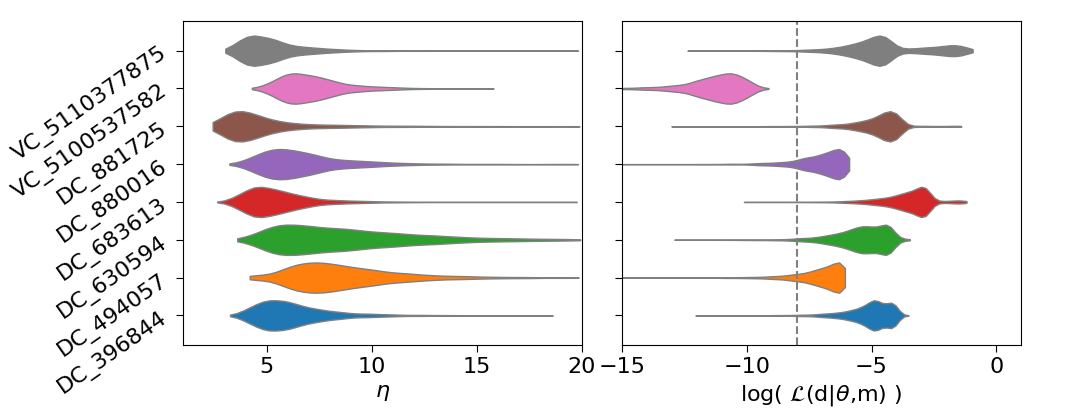
\includegraphics[width=1.0\textwidth]{plots/violin_new.png}
    \caption{\textit{Left}: violin plot representing the 1-d marginalized posterior distributions for the parameter $\eta$. Posteriors are obtained from the MCMC runs described in section \ref{sec:mcmc} \textit{Right}: violin plot representing the probability distribution associated with the natural logarithm of the likelihood term, $\log( \mathcal{L}(d|\Theta,m))$; in our setup, this term equals to $-\chi^2(d|\Theta)$. The gray dashed line shows the expectation value of $-\chi^2$ (see section \ref{sec:chi2} for more details).
    \label{fig:violin}
    }
\end{figure*}



Figure \ref{fig:corner_1} and figure \ref{fig:corner_2} show the "corner plots" for the MCMC runs described in the last section. Every set of plots refers to one of the systems of the "\CII Halo" F20 sample. Corner plots show the various combinations of 1-d and 2-d distributions of the chains $\{\Theta_i\}_{i=1}^N$ obtained from the different runs; mathematically, they represent the 1(2)-d posterior distributions obtained by marginalizing over all the parameters except for one (two) at a time.
%
Therefore, the 1-d histograms are the probability distributions for the single parameters: $\log\eta$, $\mathrm{SFR}$, and $v_c$. From these distributions, the median values and the $1\sigma$ errors (i.e., the $16^\mathrm{th}$ and $84^\mathrm{th}$ percentiles) can be obtained: these are the best estimates for the parameters that we can achieve with our data-model comparison -- they are shown at the top of every 1-d histogram in the figures.

Red shaded regions in figs. \ref{fig:corner_1}, \ref{fig:corner_2} highlight the observational bounds for $\mathrm{SFR}$ and $v_c$. All corner plots show distributions for these two parameters that are perfectly compatible with these bounds. This does not come as a surprise, since our choice for the priors biases the distributions towards the interval gauged by observations. It is interesting to note, however, that there is evidence for a bimodal shape of the posterior distribution, especially for the 1-d posterior on the $v_c$ parameter.
%
The origin of this bimodality can be investigated by looking at figure \ref{fig:mcmc_emission}: in these plots, we generate emission profiles by considering sets of values for the parameters extracted randomly from the MCMC chains. We note that two behaviors are possible: low-$v_c$ profiles form halos that are even more extended than the observational data, while higher $v_c$ values result in an emission that is less extended and barely compatible with the observed one. From the data available, there is no specific preference for any of the behaviors.

The distributions for the $\log \eta$ parameter, instead, are much more interesting, as they are not constrained by our priors choice. We show these distributions for different systems (using the parameter $\eta$ instead of $\log\eta$) in the form of a violin plot in figure \ref{fig:violin}. We obtain median values of $\eta$ in the range $\eta \approx 4-7$. These values are compatible with the ones obtained by using the $\chi^2$ test in section \ref{sec:chi2}. This implies that our Bayesian analysis supports the results we have already obtained with a simple best-fitting approach. The substantial difference lies in the fact that now we are able to assign uncertainties to the inferred values of $\eta$: we find $1\sigma$ errors of the order of $1-3$. 

Another important quantity to look at -- that cannot be easily inferred from the corner plots -- is the value of the likelihood $\mathcal{L}(d|\Theta,m)$. This quantity is relevant since it is a way to measure the "goodness of fit", i.e., the accordance between our model and the observational data. In the right panel of figure \ref{fig:violin}, we plot the probability distributions of $\log(\mathcal{L}(d|\Theta,m))$ (again using a violin plot). As pointed out in section \ref{sec:bayes}, under the hypotheses here considered, the logarithm of the likelihood is simply the inverse of the $\chi^2$. Therefore, the minimum value for $|\log(\mathcal{L}(d|\Theta,m))|$ is the result we would obtain with a $\chi^2$ test. From figure \ref{fig:violin}, we see these values are small for most of the systems, even smaller than the expected value of $\chi^2=n-1=8$ (however, see discussion in sec. \ref{sec:chi2} on the limits of the $\chi^2$ test in this context). Such small values mean that our models are good fits for the data. This can be inferred also by looking at figure \ref{fig:mcmc_emission}: most of the profiles are in very good agreement with the observational data, particularly in the internal regions, where data points have smaller relative errors. These results imply that the Bayesian approach improves our quantitative analysis substantially and that the conclusions we can draw from this model-data comparison are founded on solid grounds.

Finally, in figure \ref{fig:eta_sfr_vc}, we plot the values of $\eta$ inferred by our analysis against the observed values of the stellar mass $M_\mathrm{star}$ (left panel) and of the star formation rate (SFR) (right panel). In both these plots, we fit lines in bilogarithmic scale in order to search for power-law dependences of the form $y=a\,x^b$. 

We exclude from the fit the system DC$494057$ -- that does not belong to the "\CII Halo" class in F20 \citep{Fujimoto:2020qzo} -- because it is a clear outlier in the plots.
%
The reason for this could be the (highly) non-monotonic profile of the DC$494057$ data points: also looking at figure \ref{fig:single_profiles}, we note how our model struggles to capture the complex behavior of the external points. 

We find that both $\eta-M_\mathrm{star}$ and $\eta-\mathrm{SFR}$ are inversely correlated, with the following best-fit parameters ($\log \eta = a_\mathrm{mstar} + b_\mathrm{mstar} \log( M_\mathrm{star}/10^{10}\msun) =  a_\mathrm{SFR} + b_\mathrm{SFR} \log( \mathrm{SFR} /\msun\,\mathrm{yr}^{-1})$):
\begin{align}
    a_\mathrm{mstar} &= 5.1\pm0.4 & b_\mathrm{mstar} &= -0.38\pm0.17      \\
    a_\mathrm{SFR} &= 10.0\pm2.1 & b_\mathrm{SFR} &= -0.13\pm0.07
\end{align}
Therefore, our model suggests that mass loading factors for high-z, normal star-forming galaxies lie in the range $\eta\approx3-10$ (accounting for the statistical uncertainties), with higher values for low-mass and low-SFR systems.

\subsection{Comparison with previous works} 


It is interesting to quantitatively compare our conclusions with other previous works on galactic outflows. Despite the fact that mass loading factors cannot be constrained with high accuracy from observations (chapter \ref{chap:outflows}), there exist some estimates for $\eta$ both locally and at high-redshift that can help us to put our results in the right context.

A seminal work by \citet{Heckman15} uses UV absorption lines to study the properties of SF-driven outflows in local starburst galaxies; the authors of the study find that the mass loading factor correlates weakly and inversely both with $\mathrm{SFR}$ and $v_c$ (or, equivalently, $M_\mathrm{star}$). They identify values for $\eta$ ranging from $1 \lesssim \eta \lesssim 4$: this range of values is lower than the one we find in our study, even though there is a partial overlap. This tension may be due to the fact that hidden (faint) AGN activity may contribute to power outflows in the ALPINE galaxies. This hypothesis is appealing because AGN-driven outflows, being more powerful and disruptive, are characterized by higher values of the mass loading factors \citep[see e.g.,][]{Fiore_2017,fluetsch2019cold}. 

However, we also note that a number of other studies find values for $\eta$ that are significantly higher, and thus compatible with our conclusions. For instance, using H$\alpha$ emission lines originating in the CGM of local galaxies, \citet{zhang2021empirical} measure the mass loading factor for different ranges of halo masses. In the range we are interested in, their result is $2 \lesssim \eta \lesssim 7$, which is in very good agreement with the values we have found.

At high redshifts, the analysis of the broad-wing feature identified by G20 \citep{ginolfi:2019} in the ALPINE star-forming sample (section \ref{sec:alpine}) gives an estimate for $\eta\approx 0.5-2$. However, the HC21 work \citep{herrera2021kiloparsec} (section \ref{sec:alpine}), studying the DC$494057$ system, find similar values for the total mass loading factor only on a global level. In fact, they are also able to resolve the regions where the outflow originates and to compute local values of $\eta$; they find $\eta = 3-6$, which is compatible with our results. This also suggests that measurements of the mass loading factors could be underestimated because of the locality of outflow launching sites. 

\begin{figure*}
    \centering
    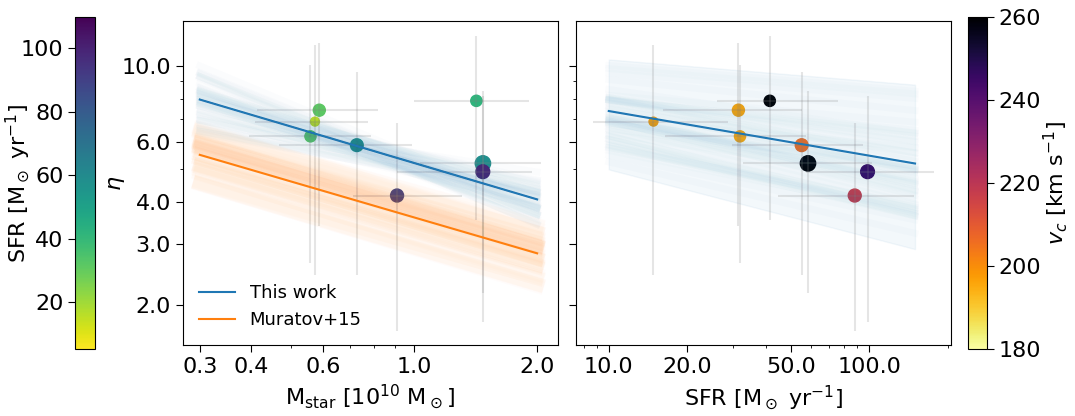
\includegraphics[width=1.0\textwidth]{plots/final_comparison_new.png}
    \caption{\textit{Left}: dependence of the mass loading factor $\eta$ on the stellar mass $M_\mathrm{star}$. The values of $\eta$ plotted are the medians and the $1\sigma$ errors of the 1-d probability distributions obtained from the MCMC analysis (figure \ref{fig:violin}). Stellar masses are inferred from observational data (table \ref{tab:alpine_sample} or figure \ref{fig:alpine_trends}). We fit a power law (i.e., a line in logarithmic scale) in blue to highlight the global trend revealed by our comparison, and we also show previous results from \citet{muratov2015} for reference. Data points are color-coded according to their SFR, as inferred from observations. The size of every point is proportional to its likelihood $\mathcal{L}(d|\Theta,m)$ (figure \ref{fig:violin}). \textit{Right}: dependence of the mass loading factor $\eta$ on the star formation rate (SFR). The same considerations as for the left panel apply. The color of the data points expresses their global circular velocity $v_c$, which is a function of the stellar mass via the SMHM relation (see section \ref{sec:sample_description} for more details). 
    \label{fig:eta_sfr_vc}
    }
\end{figure*}


Simulations have the capabilities to measure mass loading factors much more directly, as well as to study their evolution with redshift and their dependence on the properties of the galaxies. With this respect, \citet{muratov2015} uses the \code{fire} zoom cosmological simulations to study the impact of galactic winds on galaxies. They identify a power-law relation between the mass loading factor $\eta$ and the stellar mass $M_\mathrm{star}$ of the same form like the one we have obtained using our comparison with data. They find the following values for the parameters $a$ and $b$ ($\log \eta = a + b \log( M_\mathrm{star}/10^{10}\msun)$):
\begin{align}
    a &= 3.6\pm0.7 & b &= -0.36\pm0.02      
\end{align}
Figure \ref{fig:eta_sfr_vc} compares our best-fit result with the one of \citet{muratov2015}. We find very similar relations, although our values of $\eta$ are systematically higher. However, it is hard to tell whether this small difference is due to some systematical bias or it contains some interesting physical insight. As the \code{FIRE} simulations do not contain any AGN contribution, this offset could be hinting at the presence of hidden AGN activity. 

Subsequent works of \citet{mitchell2021gas} and \citet{pandya2021characterizing}, using the \code{EAGLE} and the \code{FIRE-2} simulations respectively, obtain similar trends supporting an inverse dependence of $\eta$ on $M_\mathrm{star}$.

\begin{figure*}
    \centering
    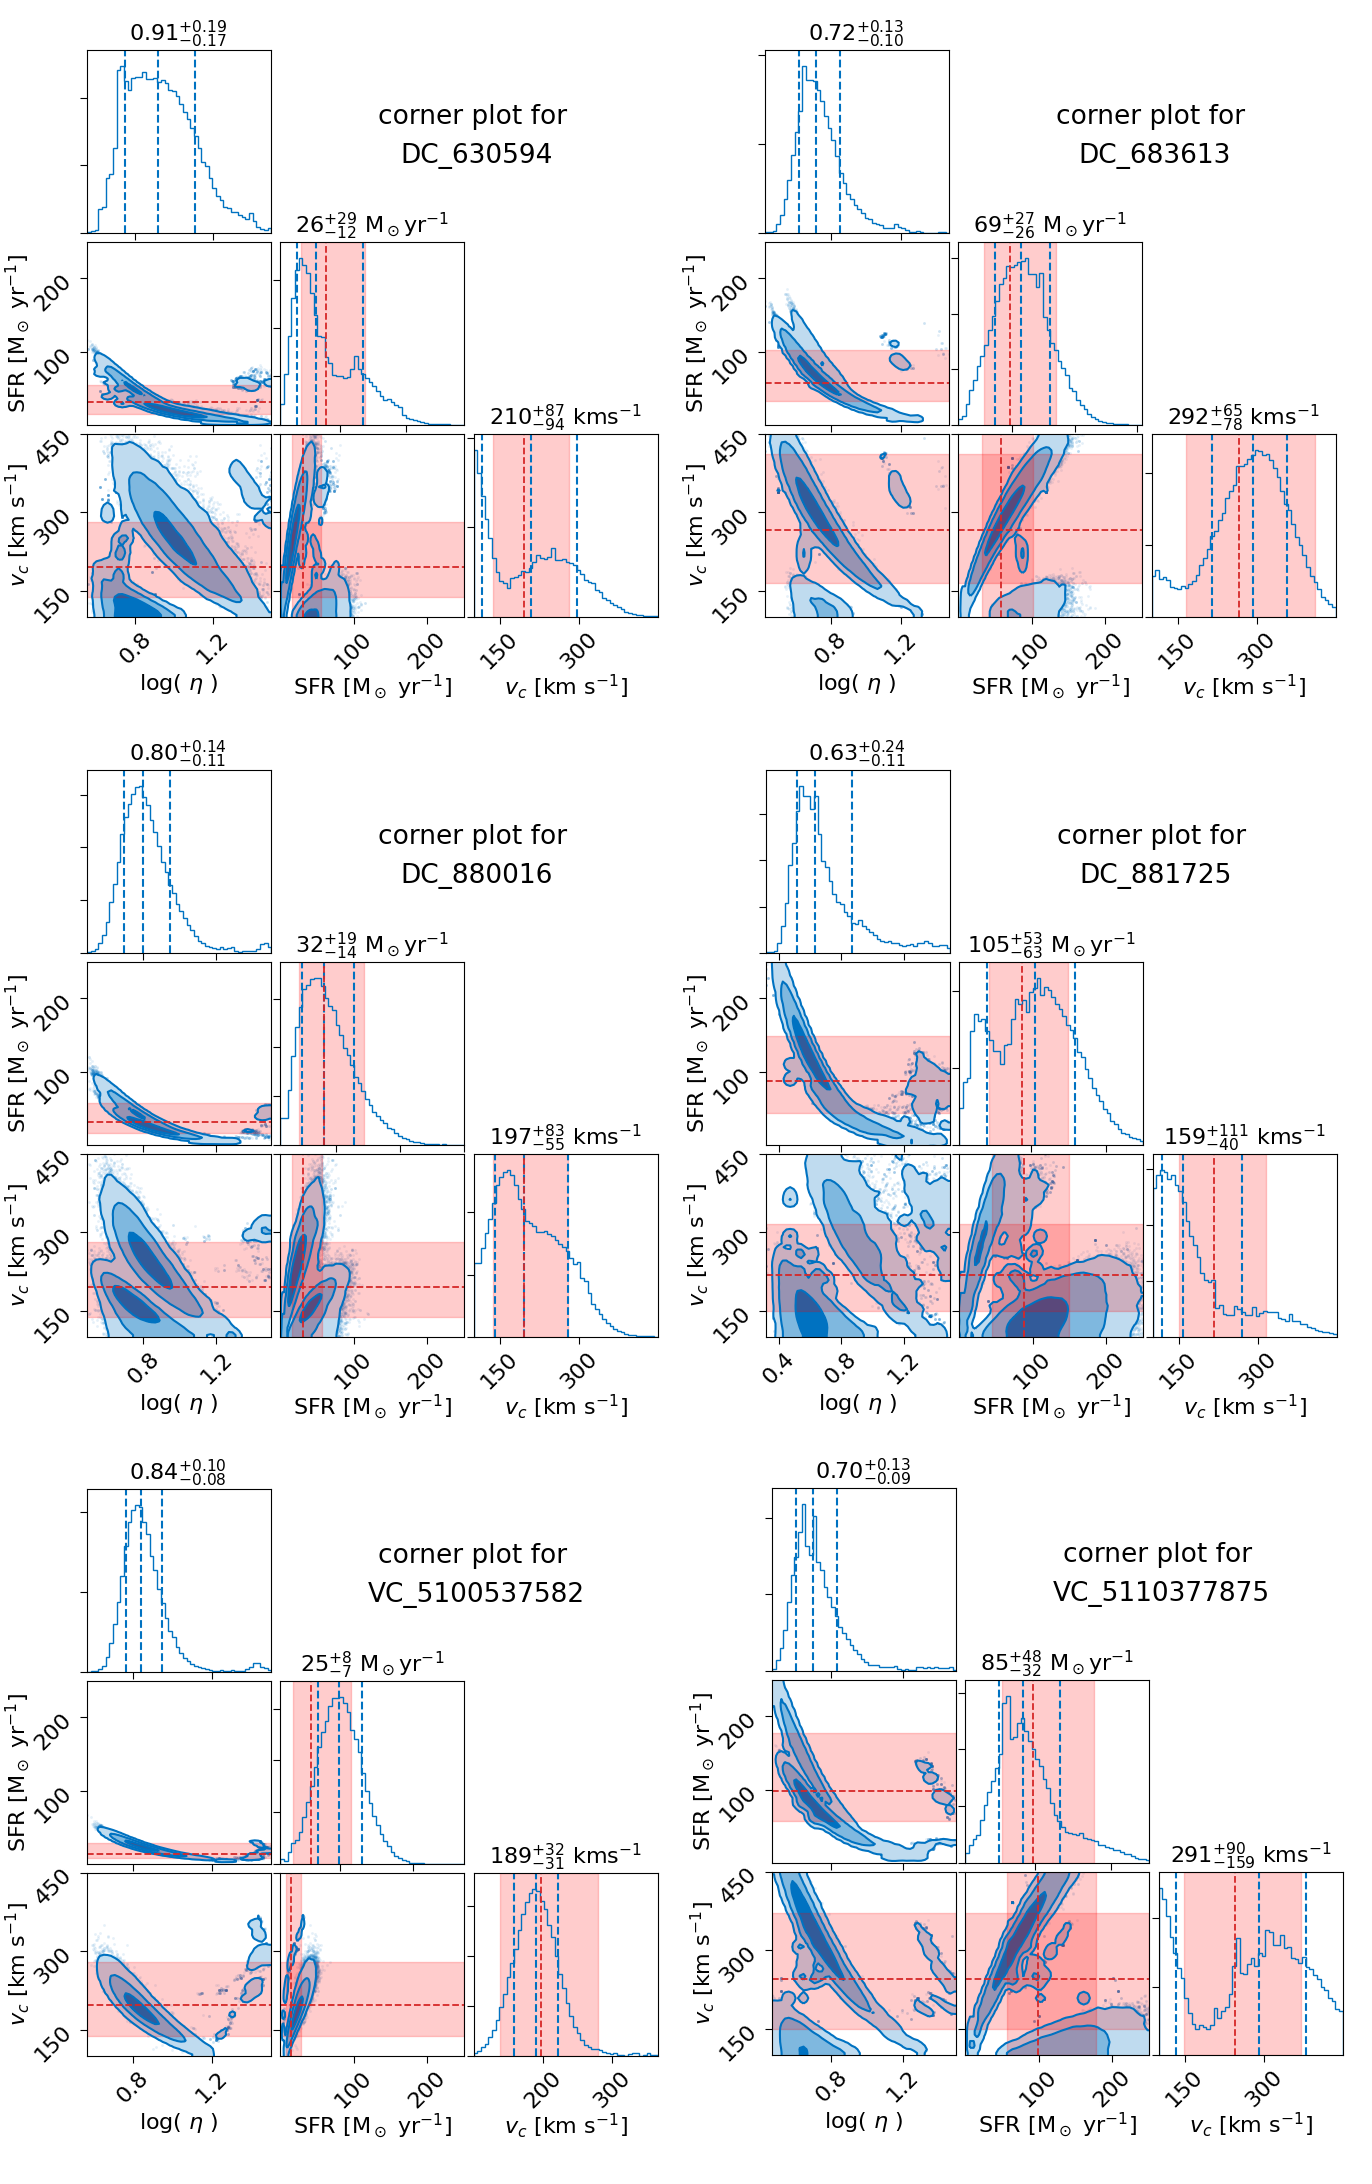
\includegraphics[width=1.0\textwidth]{plots/corner_final_2.png}
    \caption{Same as figure \ref{fig:corner_1}; the results for the rest of the data sample considered are shown here. 
    \label{fig:corner_2}
    }
\end{figure*}
